\chapter{Domain Model}

% Preface the high-level organization of the domain

At its highest level, Capital Games consists of a few subsystems
working together and coordinated by an internal controller. The
end user interacts with the application through either a web browser
or by directly submitting HTTP requests to the server. These actions
are equivalent because user actions are translated into RESTful actions
and interpreted equivalently by an appropriate RESTful controller. \cite{wiki:restful}
Once a controller is invoked, it consults the 
internal subsystems before responding to the request. Each of the 
subsystems can be identified by the purpose they serve in relation
to the application. 

% Concept Definitions
\section{Concept Definitions}

\subsection{Database}
By its nature as a data-driven site, data persistence
is core to Capital Games. Therefore, a database subsystem is necessary. 
A challenge often encountered when using databases in an application is
the translation of database-native datatypes to the more varied datatypes
employed by dynamic applications. \cite{wiki:orm} To simplify this,
Capital Games uses the ActiveRecord object-relational mapper to abstract
the logic between the database and the system as a whole. Only privileged portions
of the system have access to the database. This maintains the safety of the
data while also allowing it to be manipulated more precisely. Per the convention
of MVC-style application style architecture 
% insert reference here for later chapter
(upon which we base our application, described in more detail later), these 
are known as the Models. The database is explored in more detail in the Data Structures section.

\subsection{Finance API Adaptor}
The data for the application comes from a third party source, Yahoo! Inc. Yahoo!
provides both nearly-real-time and historical data on most U.S.-traded stocks.
Yahoo! exposes this data through a web API service in which a party can make
up to several thousand requests against Yahoo!'s databases daily. The party
simply enters arguments into an HTTP request which is interpreted by Yahoo!
as a database search, runs the query, and returns the results in CSV format. \cite{gummy}

In order to interact with the web service, we employ an adaptor plugin which
translates between the various syntaxes used by Yahoo! and our own system.
Any and all parts of the application which require access to a live data-stream
invoke the Finance Adaptor subsystem, which in turn queries Yahoo!. This
modularity enables multiple subsystems of the application to have access to live data
when necessary.

\subsection{Queueing (Asynchronous Task) System}

Fundamentally, Capital Games is about placing trading orders for various stocks. 
Though the simplest type, market orders, are executed almost immediately after being 
placed, stop and limit orders may not be executed for quite some time. \cite{inv:market}
\cite{inv:stop} \cite{inv:limit} This begs the question of how to perform a trade
at some undetermined time after the order is placed. 
Upon further inspection, a few other functions of the site depend on a similar capability.
In order to update the user portfolio database regularly or send out newsletters, the system 
must be able to asynchronously execute certain tasks. Enter a Queueing System.

Whenever a task needs to be performed asynchronously, the task is entered into a 
designated portion of a Redis database, configured as a queue. Background "workers" 
(processes) perform tasks as they arrive. Tasks can also be scheduled to occur at specific
times or intervals. In this way, everything from polling the datastream for stock updates
to performing scheduled updates and e-mails can be coordinated by a single system.

\subsection{Views Generator}

Finally, when all data have been collected and a response needs to be rendered, those data
are delivered to a subsystem which dynamically generates the content
which are served up to the end-user. The Views Generator contains various modules which
simplify translating the data to web-standard HTML and Javascript.

\subsection{Mailer System}

Capital Games is designed to periodically alert users as to their portfolio performance.
This is performed by the Queueing System in conjunction with the Mailer system.
The framework we employ natively contains a robust mailing system called Action Mailer,
which generates content dynamically at runtime. \cite{action:mailer} This allows us to perform calculations
on leagues and then include that into emails, in addition to raw data.

%\begin{itemize}
%\item \textbf{Users}: Every end-user of the application needs both a private and
%public facing identity on the site.
%
%\item \textbf{Site Administrators}: The site needs a few global administrators
%who can delete posts and ban users which are innappropriate, as well
%as perform several maintenance features.
%
%\item \textbf{Leagues}: Every end-user is participating in one or more leagues.
%
%\item \textbf{Investors}: Because an end-user can participate in multiple leagues,
%and each instance of the user can have a separate amount of money, margin,
%etc., it is necessary to maintain a separate identity for each of these 
%instances -- \emph{investors}.
%
%\item \textbf{League Manager}: Every League should have a superuser who is 
%able to invite other players, perform moderation, and change settings.
%\end{itemize}
%
%Although not actors themselves, from UC-4 (page \pageref{UC-4}) and UC-5 
%(page \pageref{UC-5}) it is apparent that end-users are implicitly 
%requesting and manipulating data for their orders and portfolios. These,
%too, become part of the application domain.
%
%\begin{itemize}
%\item \textbf{Orders}: When an \emph{Investor} places any type of order, it
%needs to be tracked. 
%\item \textbf{Stocks}: Whenever an Investor is tracking the performance of a
%stock, those data need to be stored locally. Stocks is a unified 
%data object to contain those data.
%\end{itemize}
%
%One of the actors at the back end of UC-3 (page \pageref{UC-3}) and UC-4
%(\pageref{UC-4}) was the Financial API, responsible for accessing the 
%market data stream. 
%
%\begin{itemize}
%\item \textbf{Financial API}: This module presents an interface for requesting market
%data, both live and historical. 
%\end{itemize}
%
%Upon further analysis, it becomes apparent that the domain model is missing
%functionality responsible for asynchronously executing jobs. This is another
%core feature of the site, without which Stop and Limit Orders could not 
%be placed.
%
%\begin{itemize}
%\item \textbf{Queueing System}: Many interactions need to be performed asynchronously,
%such as the execution of Stop and Limit Orders and the delivery of e-mail 
%updates. This module encapsulates the functionality of creating, maintaining,
%and executing jobs which need to be performed asynchronously.
%\end{itemize}
%
%Finally, we need an abstraction for the part of the system which invokes and operates
%upon the rest as a collective.
%
%\begin{itemize}
%\item \textbf{Controller}: The Controller is the model which receives requests from 
%the end-user, interprets them, invokes other models and modules accordingly, and 
%returns the response (when applicable).
%\end{itemize}
%
%
%% Association definitions between actors
\section{Association Definitions}

As indicated in Figure~\ref{domainModel2}, there are 6 components which are core
to our system: Controller, Views, Models, Finance Adaptor, Queueing System, and
Mailer.

The Controller acts as the single point-of-entry for all user interactions. It
interpretes requests and accordingly accesses the Models, the Finance Adaptor,
and the Queueing System, before delivering the necessary data to the Views
Generator. By definition, the Controller is the most prviliged system component.

The Queueing System is possibly more privileged than the Controller. It has a great deal
of autonomy, functioning without the Controller and being able to invoke other systems
on its own. Compare this to the Controller, which is only invoked upon requests from
a user. The Queueing System communicates with Models, the Finance Adaptor, and the 
Mailer as necessary to perform its tasks.

Conversely, the Views Generator is the least privileged subsystem. It cannot
externally communicate and only responds to to the actor which called it.

The Finance Adaptor, Mailer, and Models are each afforded limited privileges, in that the
Models and Mailer need to communicate with the database and Views, respectively, 
while the Finance Adaptor needs to communicate with external data sources through the Internet.
They each respond directly to requests from the componenets which invoke them.

\begin{figure}
\centering
\label{domainModel2}
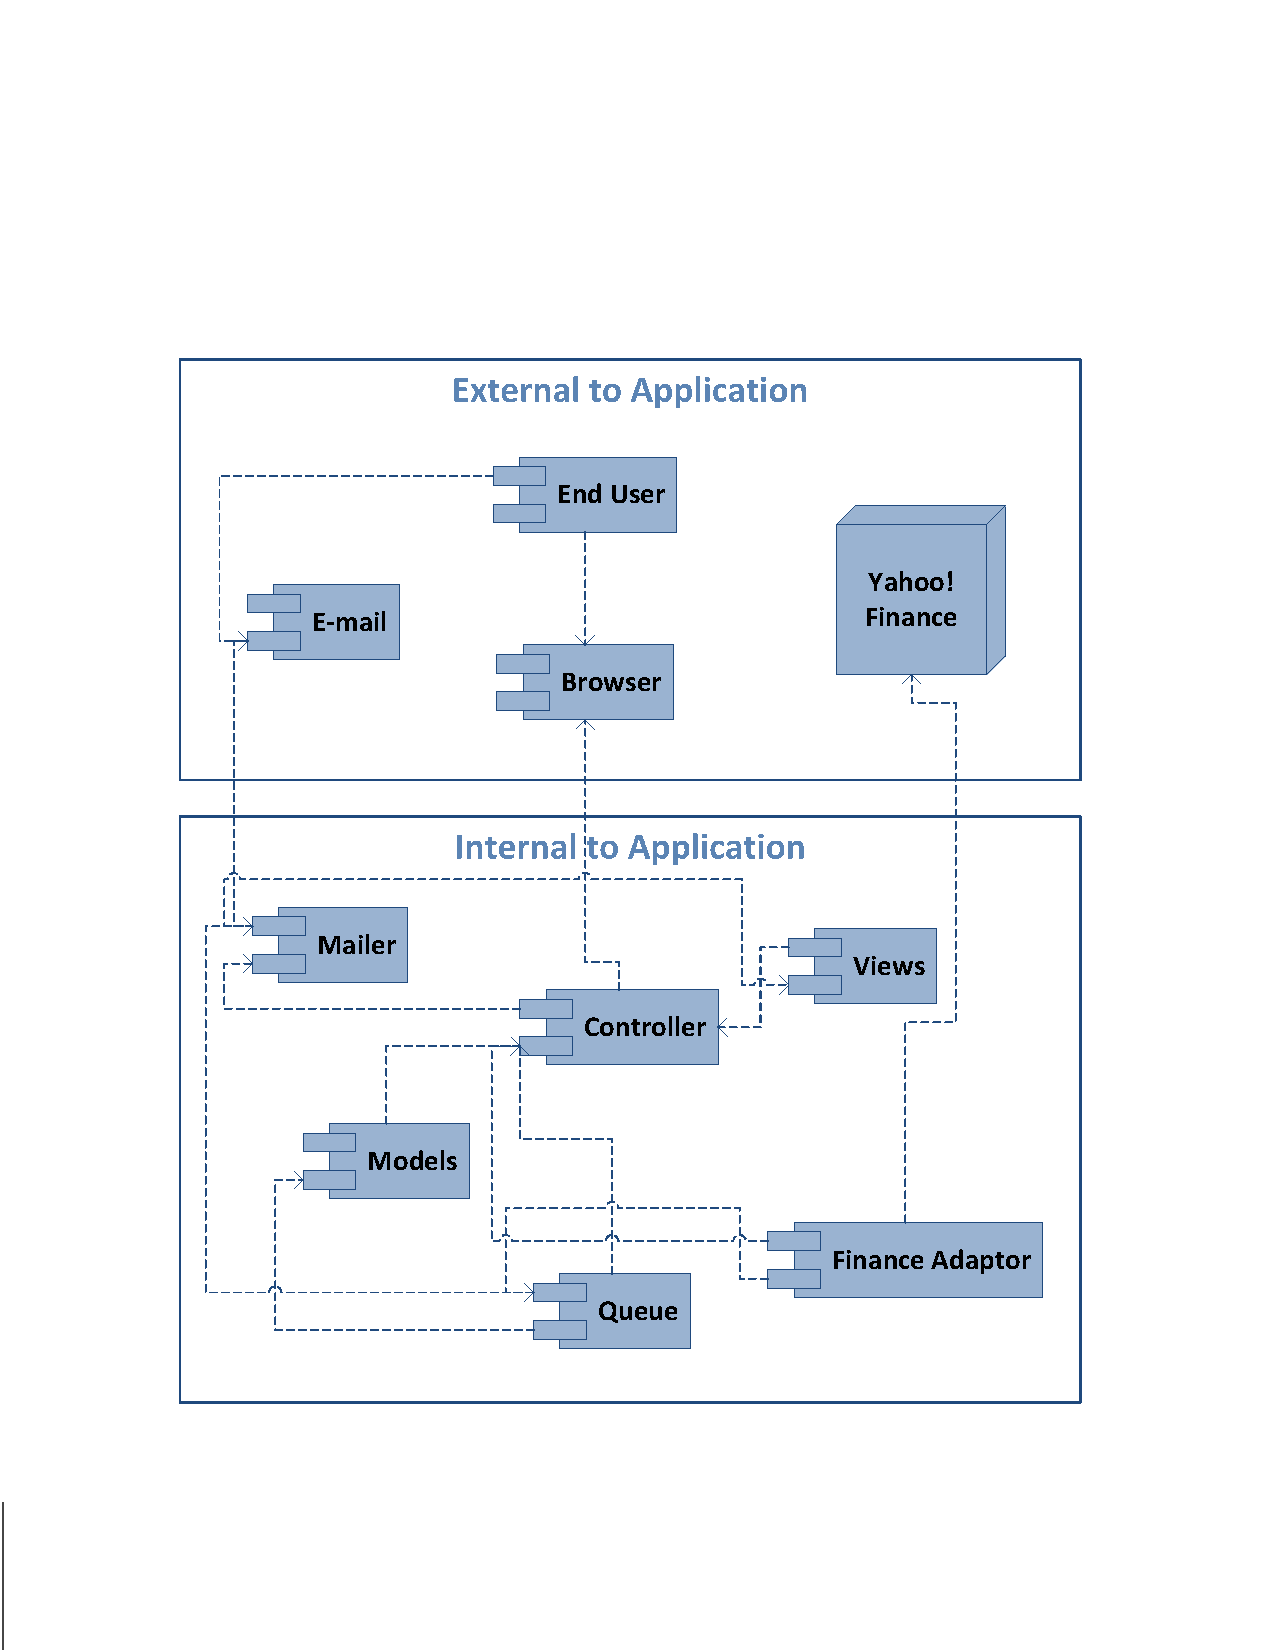
\includegraphics[width=6.5in]{./img/domainModel2.pdf}
\caption{This high-level overview of the domain model of our application shows the 
separation between the external actors User, Browser, and Yahoo! Finance, as well as
how the internal component subsystems relate to each other.}
\end{figure}
%
%% brief discussion of how the parts relate to each other
%Clearly, many of these models are interrelated. Below is a non-comprehensive
%list of associations between various types of models.
%
%\begin{itemize}
%\item \textbf{Controller}: The Controller interacts with the collective database layer, 
%as well as the other core modules.
%	\begin{itemize}
%	\item \textbf{Association}: Controller invokes the Database layer (and data contained therein)
%	\item \textbf{Association}: Controller invokes the Financial API 
%	\item \textbf{Association}: Controller invokes the Queueing System
%	\end{itemize}
%\item \textbf{Queuing System}: The Queueing System can almost be thought of as a 
%miniature, self-regulating Controller. It can invoke the Financial API and the 
%collective database layer.
%	\begin{itemize}
%	\item \textbf{Association}: Queueing System invokes the Financial API
%	\item \textbf{Association}: Queueing System invokes the Database layer
%	\end{itemize}
%\item \textbf{Database Layer}: The Database Layer stores data into data objects and then
%saves them to the underlying database. The Database Layer can perform limited checking
%and updating logic when invoked, but is not self-regulating. It contains models of
%several types of actors.
%	\begin{itemize}
%	\item \textbf{Users}: Represents end-users and their personal information
%		\begin{itemize}
%		\item \textbf{Inheritance}: Users is the parent class of Site Administrators
%		\item \textbf{Aggregation}: Users have many Investors (User-Instances)
%		\item \textbf{Composition}: Leagues have many Users
%		\end{itemize}
%	\item \textbf{Site Administrators}: A superclass of Users
%		\begin{itemize}
%		\item \textbf{Inheritance}: Site Administrators inherits from Users
%		\end{itemize}
%	\item \textbf{Leagues}: Represents simulation instances
%		\begin{itemize}
%		\item \textbf{Composition}: Leagues have many Users
%		\item \textbf{Composition}: Leagues have many Investors (User-Instances)
%		\item \textbf{Aggregation}: Leagues have many Orders
%		\end{itemize}
%	\item \textbf{Investors}: Represents User-Instances within Leagues
%		\begin{itemize}
%		\item \textbf{Composition}: A League has many Investors
%		\item \textbf{Aggregation}: A User has many Investors
%		\item \textbf{Aggregation}: An Investor has many Orders
%		\end{itemize}
%	\item \textbf{League Managers}: A superclass of Investors
%		\begin{itemize}
%		\item \textbf{Inheritance}: League Managers inherits from Investors
%		\end{itemize}	
%	\item \textbf{Orders}: Contains order data
%		\begin{itemize}
%		\item \textbf{Aggregation}: Leagues have many Orders
%		\item \textbf{Aggregation}: Investors have many Orders
%		\item \textbf{Association}: Orders are placed for Stocks
%		\end{itemize}
%	
%		In addition, there are a few interesting types of orders, namely:
%		\begin{itemize}
%		\item \textbf{Market Order}: Orders executed immediately
%		\item \textbf{Stop Order}: Orders executed after a certain price is exceeded
%		\item \textbf{Limit Order}: Orders executed strictly beyond a certain price
%		\end{itemize}
%	\item \textbf{Stocks}: Contains data on stocks held by Investors
%		\begin{itemize}
%		\item \textbf{Association}: Orders are placed for stocks
%		\end{itemize}
%	\end{itemize}
%\end{itemize}
%

% Attribute definitions
\section{Attribute Definitions}

Though the application is a whole is not entirely object-oriented,
and thus not all parts (ie the Controller) have true attributes,
the Models, Queueing System, and Financial Adaptor all do. 

Models possess basic attributes for the data they contain, such
as user names, email addresses, stocks possessed, etc. These are
contained in Figure~\ref{domainModel}.  Similarly, Orders to
be performed in the Queue have similar identifiers, as shown in 
Figure~\ref{queuestruct}.

Validation on the data saved by the Models layer is performed 
automatically by the object-relational mapper, which can enforce
data typing rules built into the database. This happens automatically.

Orders data is proxied through the database, and so its data is also
validated before being entered. Though a remote edge case is the 
possibility of an order being valid while placed but being invalidated
(for example by a stock no longer being on the market) while in the
queue, we do not consider it at this time.

The Queueing System utilizes entities called ``background workers''.
As the name implies, these are persistent entities which wait
for work in the form of queued tasks to hit the Redis database. When
this happens, the first available worker pulls the task from the queue.

The Financial Adaptor possesses a set of financial metrics, a brief
list of which is tabulated in Table~\ref{financeparams}. When
data is retrieved by the adaptor, it is tabulated with some of the
parameters shown in the table. 


\begin{figure}
\label{queuestruct}
\centering
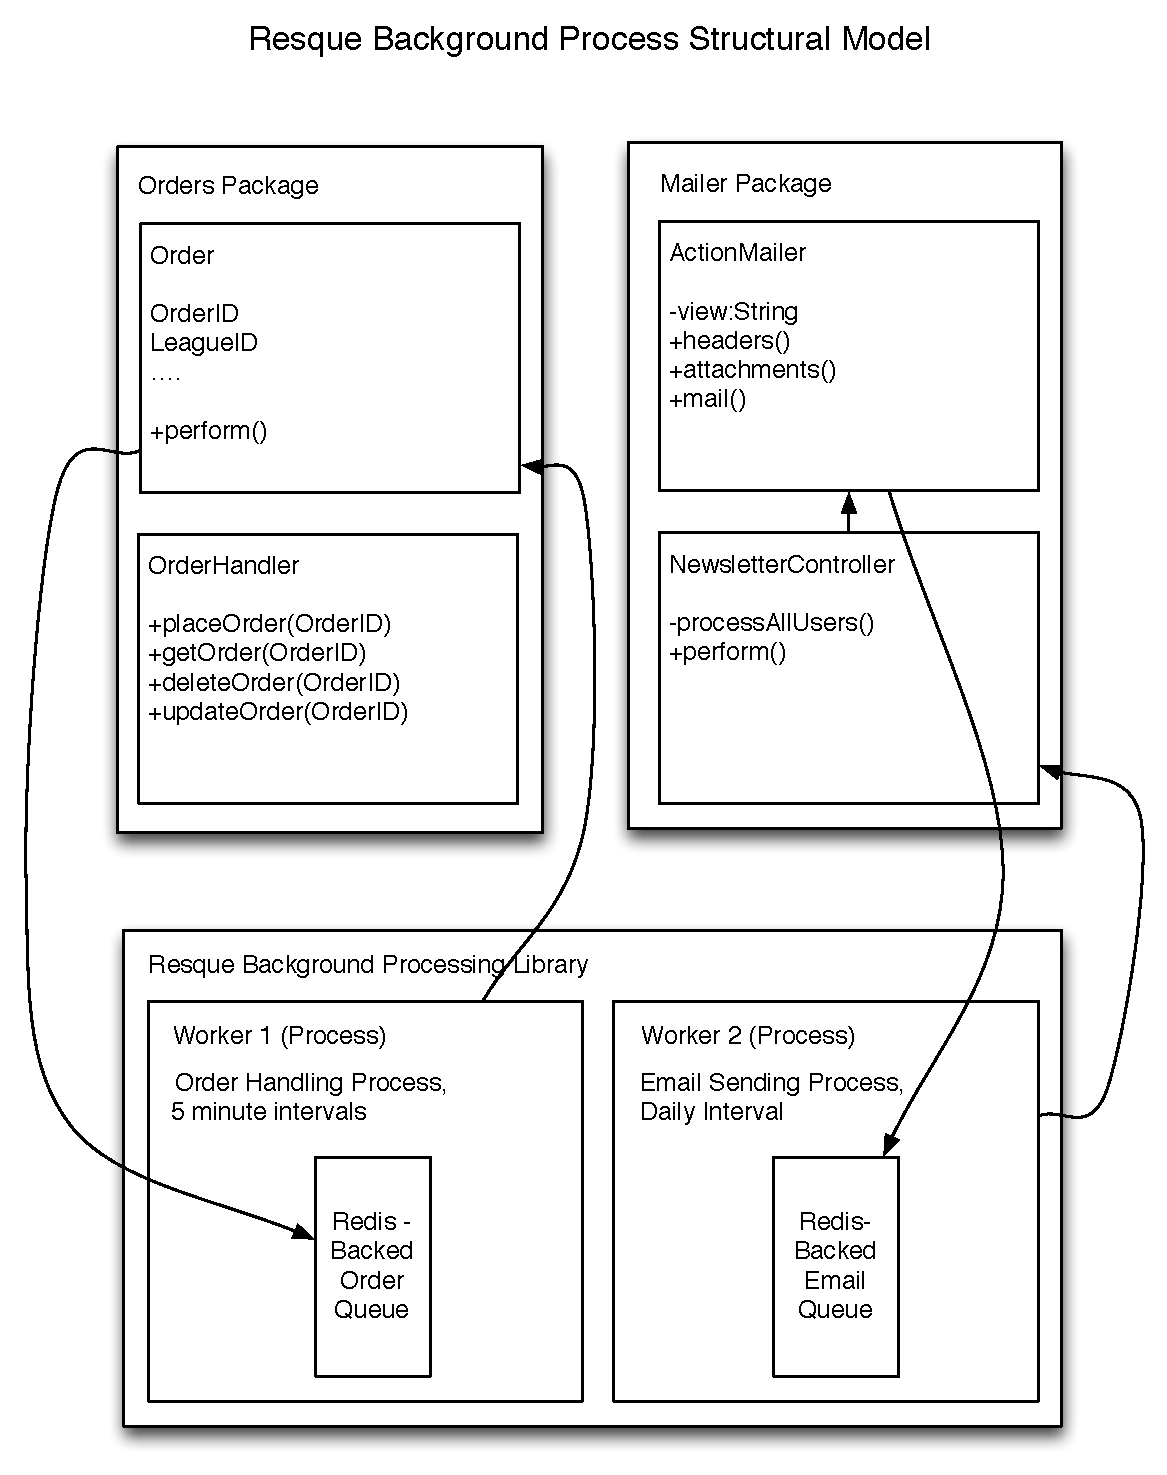
\includegraphics[width=6.5in]{./Diagrams/ComponentModels/BackgroundProcessStructuralModel.pdf}
\caption{The structural model of the Resque Queueing System. Market Orders to be placed are 
bundled as Orders and served to the queue to be processed every few minutes. Newsletters are 
performed daily and bundled and served every night. Background workers wait for updates to
the Redis database and upon seeing a valid task, pull it and begin processing.}
\end{figure}

\begin{table}
\label{financeparams}
\centering
\renewcommand\arraystretch{1.5}
\begin{tabular}{|c|c|c|c|}
\hline
Ticker & Name & Date & Time \\
\hline
Change \% & Previous Close & Open & Volume \\
\hline
Day High & Day Low & Day Range & Ticker Trend \\
\hline
Bid & Ask & Average Daily Volume & Price-to-Earnings Ratio \\
\hline
\end{tabular}
\caption{These are some of the data that Yahoo! Finance provides upon request, and which the adaptor we employ
can convert.}
\end{table}
%

%
%It is clear from the domain model abstraction above that the Database Layer
%models have many noteworthy attributes, and are heavily state-based. However,
%the Financial API has no state, and is simply an aggregation of functionality.
%Likewise with the Controller. Therefore, attributes are only elaborated on for
%the Database Layer. 
%
%\begin{itemize}
%	\item \textbf{User}
%		\begin{itemize}
%		\item Name: String
%		\item E-mail: String
%		\item Password: String
%		\item Admin: Bool
%		\item Banned: Bool
%		\end{itemize}
%	\item \textbf{Investor}
%		\begin{itemize}
%		\item Manager: Bool
%		\item League ID: Integer
%		\item User ID: Integer
%		\item Capital: Double
%		\item Margin: Double
%		\end{itemize}
%	\item \textbf{League}
%		\begin{itemize}
%		\item Start Date: Date
%		\item End Date: Date
%		\item Capital: Double
%		\item Margin: Double
%		\item Commission: Double
%		\item Privacy: Bool \footnote{To simplify joining private leagues, 
%			we allow that whenever a User is ``invited'' to join one,
%			an \emph{Investor} is created for them within that league, 
%			granting immediate access.}
%		\end{itemize}
%	\item \textbf{Orders}
%		\begin{itemize}
%		\item League ID: Integer
%		\item Investor ID: Integer
%		\item Time Ordered: Date
%		\item Time Executed: Date
%		\item Ticker: String
%		\item Order Type: String \footnote{Market, Stop, Limit}
%		\item Transaction Type: String \footnote{Buy, Sell, Short, Cover}
%		\item Quantity: Integer
%		\item Duration Valid: Date
%		\end{itemize}
%	\item \textbf{Stocks}
%		\begin{itemize}
%		\item Date: Date
%		\item Ticker: String
%		\item Price: Double \footnote{Any other interesting metrics can likewise
%			be stored here.}
%		\end{itemize}
%\end{itemize}
%
%The Queueing System itself is an aggregation of functionality
%present in the controller and operates on state data from the Database. However,
%it is still under active development, and so a model for it has not yet been 
%constructed. It could be one large, all-encompassing system, or (more likely)
%will be split off into individual subsystems.

% put some BS here...

% Traceability Matrix
% This section can be implemented at your discretion,
% and to the extent you desire. We were already
% kind of waived out of having one, but maybe include
% the derivations of the domain model from the use cases
% or at least why an MVC style works. No need to go into
% too much detail about MVC though, because there's an
% architecture report due next week anyway...
% \section{Traceability Matrix}

% Put the Domain Model Graphic here: